\documentclass{article}
\usepackage{amsmath}
\usepackage{amsfonts}
\usepackage{pgfplots}  
\usepackage{titling}  
\usepackage{blindtext}
\usepackage{enumitem}
\usepackage{tasks}
\usepackage[a4paper, total={6in, 9in}]{geometry} 
\usepackage{tikz}
\usetikzlibrary{angles, quotes}
\usetikzlibrary{shapes.geometric}

\pgfplotsset{compat=newest}

% \title{\Huge}
\begin{document}
\begin{center}
    \LARGE{I Olimpiadas de Matemáticas Colegio Real Royal School}
    \\~\\
    \large{Prueba escrita categoría euler (9°, 10° y 11°)}
    \\~\\
    \large{28 de Marzooo de 2025}
\end{center}
\section{Instrucciones e Información}
\begin{itemize}
    \item No inicie la prueba hasta que la persona a cargo lo indique
    \item Esta prueba tiene preguntas cerradas y abiertas, solo es necesario argumentar las preguntas
          abiertas.
    \item En caso de que la pregunta sea abierta, asegúrese de escribir claramente la respuesta final en la hoja de respuestas.
    \item Las preguntas cerradas solo es necesario marcar la opción deseada en la hoja de respuestas.
    \item Los diagramas no están necesariamente dibujados a escala, se ofrecen únicamente como ayudas visuales.
    \item Se permite el uso de papel para operaciones, papel cuadriculado, regla y compás. No se
          permite ninguna otra ayuda.
    \item Tendrá exactamente 60 minutos para completar el mayor número de preguntas.
\end{itemize}
\section{Prueba escrita}
\begin{enumerate}
    \item{Sea ABCDEF un hexágono regular, y G el punto medio del segmento BC, ¿Cuál es la razón del área del triángulo AGH y el trapecio EHIF? \\ \begin{center}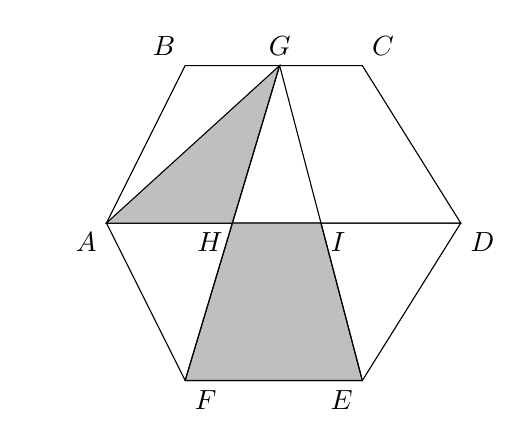
\begin{tikzpicture}
                  \coordinate (A) at (0,0);
                  \coordinate (B) at (1,2);
                  \coordinate (C) at (3.25,2);
                  \coordinate (D) at (4.5,0);
                  \coordinate (F) at (1,-2);
                  \coordinate (E) at (3.25,-2);
                  \coordinate (G) at (2.2,2);
                  \coordinate (H) at (1.6,0);
                  \coordinate (I) at (2.725,0);
                  \node[draw=none,minimum size=2cm,regular polygon,regular polygon sides=6] (a) {};
                  % Draw the outer shapes with outline
                  \draw[black] (A) -- (B) -- (C) -- (D) -- cycle;
                  \draw[black] (A) -- (F) -- (E) -- (D) -- cycle;

                  % Fill the triangular shapes with opacity and outline
                  \draw[black, fill=gray!50] (A) -- (G) -- (H) -- cycle;
                  \draw[black, fill=gray!50] (F) -- (H) -- (I) -- (E) -- cycle;
                  \draw[black, fill=gray!50] (F) -- (G);
                  \draw[black, fill=gray!50] (E) -- (G);
                  % Add angle measures
                  %   \pic [draw, angle radius=6mm, "$\alpha$", angle eccentricity=1.3] {angle = H--A--G};
                  %   \pic [draw, angle radius=6mm, "$\beta$", angle eccentricity=1.3] {angle = G--E--F};
                  %   \pic [draw, angle radius=6mm, "$\gamma$", angle eccentricity=1.2] {angle = C--D--F};

                  % Label points (optional)
                  \foreach \point/\position in {A/below left, B/above left, C/above right, D/below right, E/below left, F/below right, G/above, H/below left, I/below right}
                  \node[\position] at (\point) {$\point$};
              \end{tikzpicture}\end{center}}
    \item Si $a + b = 10$ y $a^2 + b^2 = 50$, ¿a cuanto equivale $ab$?
    \item Sea $f$ una función tal que $f(x + y) = f(x) + f(y)$ para todo $x, y \in \mathbb{R}$. Hallar el valor de  $f(0) + f(1) + f(2) + f(3)$ si $f(1) = 1/2$.
    \item{Si un círculo de diámetro 10 es dividido en muchas secciones y luego reorganizado para formar un rectángulo, ¿cuánto es la diferencia del perímetro del rectángulo y la circunferencia original del círculo?
          %   \\    \begin{center}
              
          %   \end{center}
        }
    \item Thor tiene siete rocas y un martillo. Cada vez que le pega a una roca con su martillo, se parte en cinco rocas más pequeñas. Si parte las rocas varias veces, ¿cual de los siguientes números puede ser el número de rocas que obtiene al final? \\ \begin{tasks}[label=\Alph*.](5)
              \task 17
              \task 20
              \task 21
              \task 23
              \task 25
          \end{tasks}
    \item El resultado de $1-2+3-4+5-6+...+97-98+99-100$ es igual a: \\ \begin{tasks}[label=\Alph*.](5)
              \task 0
              \task 1
              \task 50
              \task -50
              \task 101
          \end{tasks}
    \item ¿Cuántos dígitos tiene el número $4^8 * 5^{13}$? \\ \begin{tasks}[label=\Alph*.](5)
              \task 12
              \task 13
              \task 14
              \task 15
              \task N/A
          \end{tasks}
    \item{La siguiente figura consta de una circunferencia de 1 cm de radio con un cuadrado inscrito en ésta. Teniendo en cuenta que E es el punto medio del segmento DC, el área de la región de la sombreada es: \\ \begin{center} 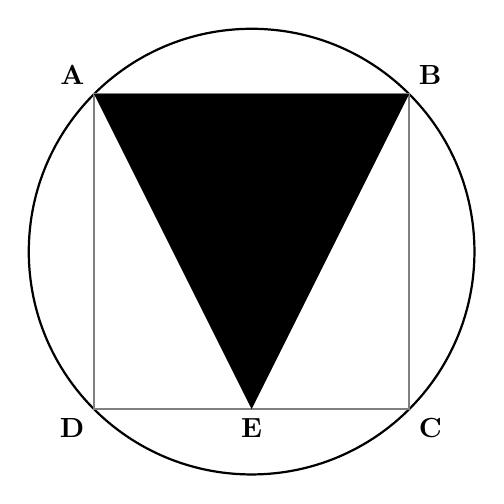
\begin{tikzpicture}
                  % Define points
                  \coordinate (A) at (-2,2);
                  \coordinate (B) at (2,2);
                  \coordinate (C) at (2,-2);
                  \coordinate (D) at (-2,-2);
                  \coordinate (E) at (0,-2);

                  % Draw circle
                  \draw[thick] (0,0) circle(2.83);

                  % Draw square
                  \draw[gray, thick] (A) -- (B) -- (C) -- (D) -- cycle;

                  % Draw inverted triangle
                  \fill[black] (A) -- (B) -- (E) -- cycle;

                  % Labels
                  \node[anchor=south east] at (A) {\textbf{A}};
                  \node[anchor=south west] at (B) {\textbf{B}};
                  \node[anchor=north west] at (C) {\textbf{C}};
                  \node[anchor=north east] at (D) {\textbf{D}};
                  \node[anchor=north] at (E) {\textbf{E}};

              \end{tikzpicture}
          \end{center}}
    \item ¿Cuál es el valor de n?  \\~\\ $7n-6n=(7+6)(7^2+6^2)(7^4+6^4)(7^8+6^8)(7^{16}+6^{16}).....(7^{2048}+6^{2048})$
    \item ¿Cuál es el valor de la siguiente ecuación? \\~\\ $\sqrt{4+\sqrt{4+\sqrt{4+\sqrt{4+...}}}}$



\end{enumerate}

\end{document}